\hypertarget{a00002}{
\section{Dokumentacja klasy MD5}
\label{d7/d46/a00002}\index{MD5@{MD5}}
}
{\tt \#include $<$md5.h$>$}

\subsection*{Metody publiczne}
\begin{CompactItemize}
\item 
void \hyperlink{a00002_72b35c041cb6983aaa74e2f1c31d5a29}{MD5Init} (\hyperlink{a00003}{MD5\_\-CTX} $\ast$)
\item 
void \hyperlink{a00002_a59116f0a26354a217fa186a43cd9d28}{MD5Update} (\hyperlink{a00003}{MD5\_\-CTX} $\ast$, unsigned char $\ast$, unsigned int)
\item 
void \hyperlink{a00002_98039031d87c1f5b787050e2b487d83f}{MD5Final} (unsigned char\mbox{[}16\mbox{]}, \hyperlink{a00003}{MD5\_\-CTX} $\ast$)
\item 
\hyperlink{a00002_fa6155ec36de415ab2dcf5e54b670d13}{MD5} ()
\end{CompactItemize}
\subsection*{Metody prywatne}
\begin{CompactItemize}
\item 
void \hyperlink{a00002_849ad3347bad15a23f3a40452476b1e0}{MD5Transform} (unsigned long int state\mbox{[}4\mbox{]}, unsigned char block\mbox{[}64\mbox{]})
\item 
void \hyperlink{a00002_c3c05716498203127920ba78b3ae8115}{Encode} (unsigned char $\ast$, unsigned long int $\ast$, unsigned int)
\item 
void \hyperlink{a00002_ef62580b93f2122c62493464787b814a}{Decode} (unsigned long int $\ast$, unsigned char $\ast$, unsigned int)
\item 
void \hyperlink{a00002_76c181f092e81df65dadf8861272ac80}{MD5\_\-memcpy} (\hyperlink{a00010_73204e40637f83518fb695362ea084a4}{POINTER}, \hyperlink{a00010_73204e40637f83518fb695362ea084a4}{POINTER}, unsigned int)
\item 
void \hyperlink{a00002_e1a522aab83da49d1bd3f0a6f3edcd11}{MD5\_\-memset} (\hyperlink{a00010_73204e40637f83518fb695362ea084a4}{POINTER}, int, unsigned int)
\end{CompactItemize}


\subsection{Opis szczegółowy}


Definicja w linii 60 pliku md5.h.

\subsection{Dokumentacja konstruktora i destruktora}
\hypertarget{a00002_fa6155ec36de415ab2dcf5e54b670d13}{
\index{MD5@{MD5}!MD5@{MD5}}
\index{MD5@{MD5}!MD5@{MD5}}
\subsubsection[{MD5}]{\setlength{\rightskip}{0pt plus 5cm}MD5::MD5 ()\hspace{0.3cm}{\tt  \mbox{[}inline\mbox{]}}}}
\label{d7/d46/a00002_fa6155ec36de415ab2dcf5e54b670d13}




Definicja w linii 77 pliku md5.h.

\subsection{Dokumentacja funkcji składowych}
\hypertarget{a00002_ef62580b93f2122c62493464787b814a}{
\index{MD5@{MD5}!Decode@{Decode}}
\index{Decode@{Decode}!MD5@{MD5}}
\subsubsection[{Decode}]{\setlength{\rightskip}{0pt plus 5cm}void MD5::Decode (unsigned long int $\ast$ {\em output}, \/  unsigned char $\ast$ {\em input}, \/  unsigned int {\em len})\hspace{0.3cm}{\tt  \mbox{[}private\mbox{]}}}}
\label{d7/d46/a00002_ef62580b93f2122c62493464787b814a}




Definicja w linii 293 pliku md5.cpp.

Here is the caller graph for this function:\nopagebreak
\begin{figure}[H]
\begin{center}
\leavevmode
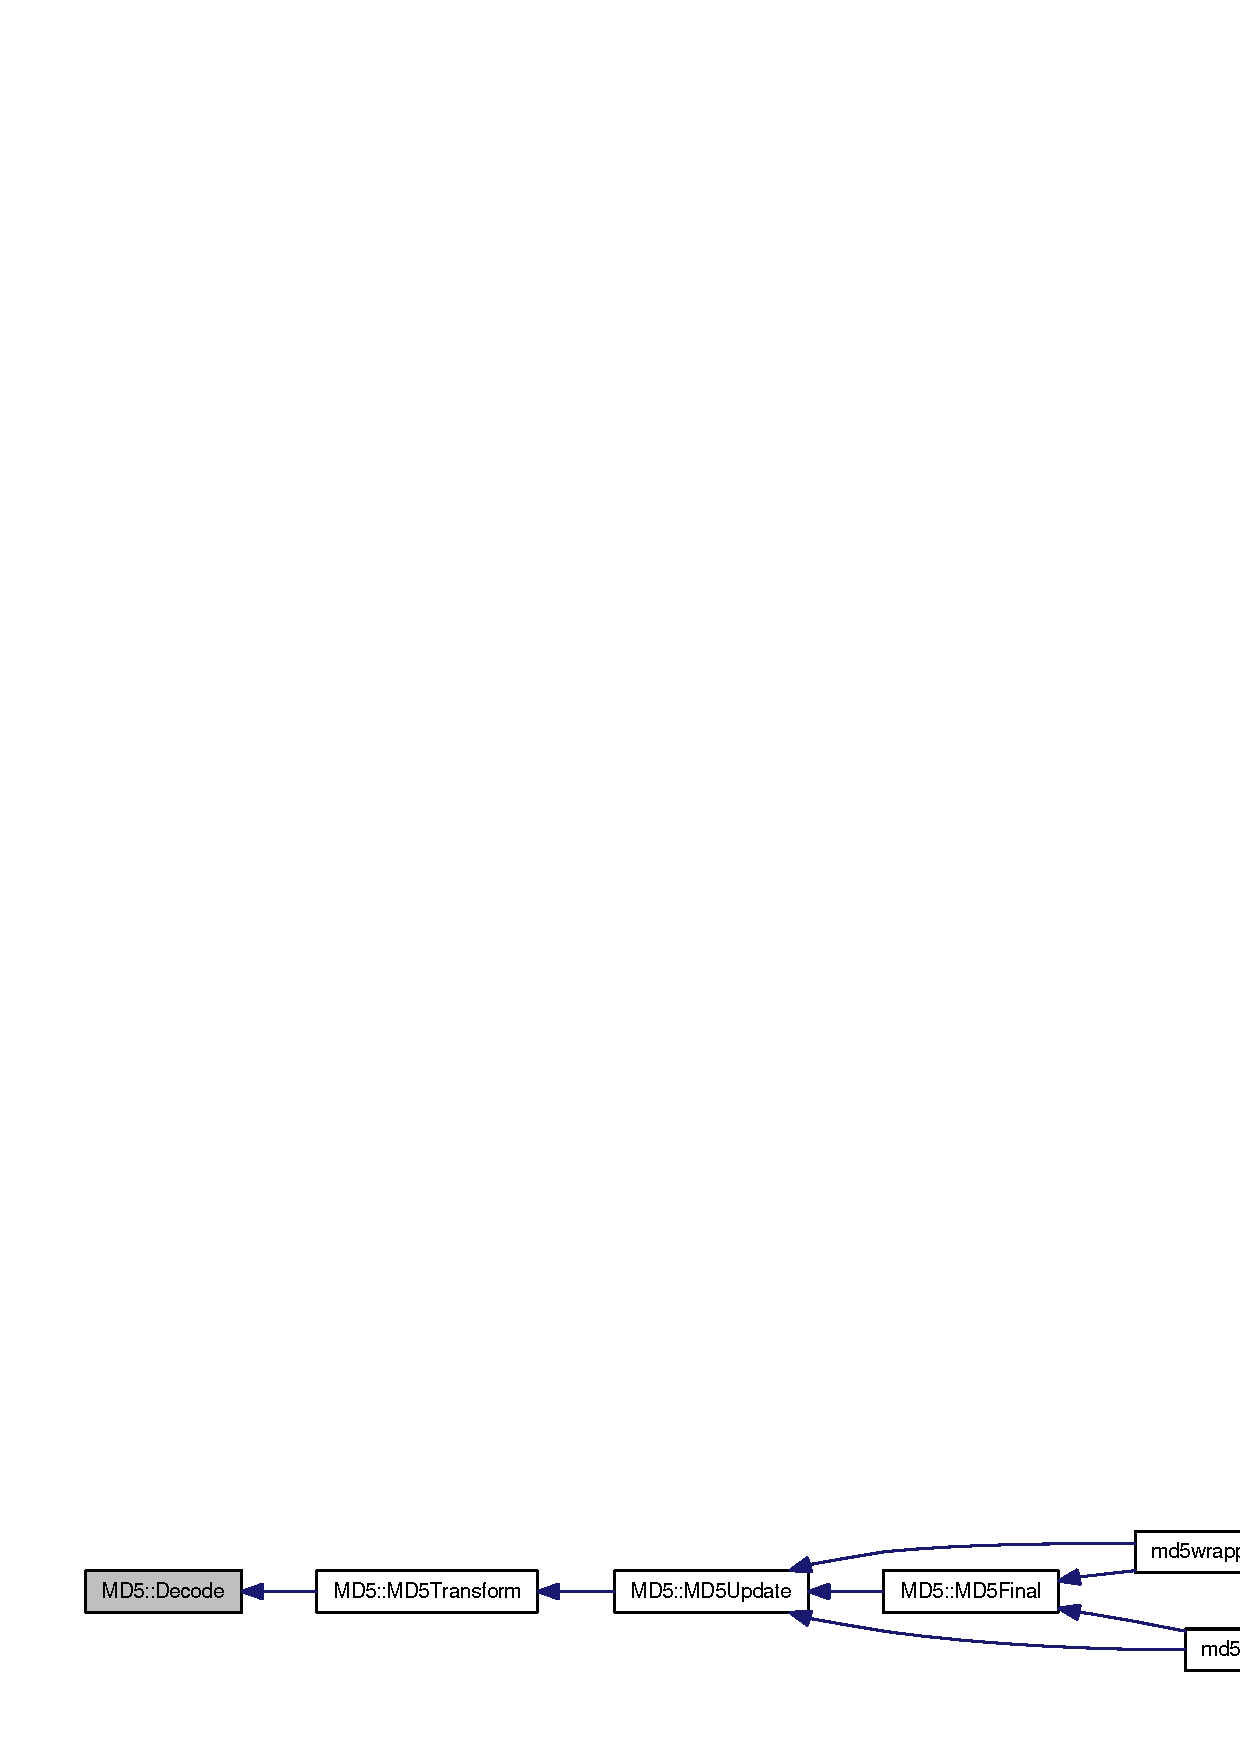
\includegraphics[width=420pt]{d7/d46/a00002_ef62580b93f2122c62493464787b814a_icgraph}
\end{center}
\end{figure}
\hypertarget{a00002_c3c05716498203127920ba78b3ae8115}{
\index{MD5@{MD5}!Encode@{Encode}}
\index{Encode@{Encode}!MD5@{MD5}}
\subsubsection[{Encode}]{\setlength{\rightskip}{0pt plus 5cm}void MD5::Encode (unsigned char $\ast$ {\em output}, \/  unsigned long int $\ast$ {\em input}, \/  unsigned int {\em len})\hspace{0.3cm}{\tt  \mbox{[}private\mbox{]}}}}
\label{d7/d46/a00002_c3c05716498203127920ba78b3ae8115}




Definicja w linii 277 pliku md5.cpp.

Here is the caller graph for this function:\nopagebreak
\begin{figure}[H]
\begin{center}
\leavevmode
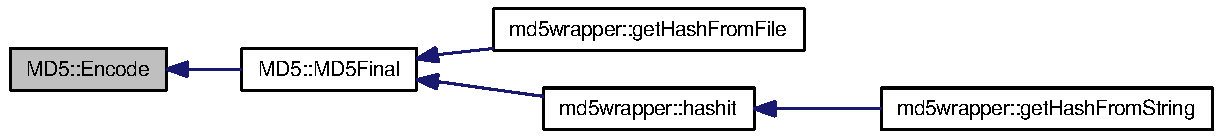
\includegraphics[width=311pt]{d7/d46/a00002_c3c05716498203127920ba78b3ae8115_icgraph}
\end{center}
\end{figure}
\hypertarget{a00002_76c181f092e81df65dadf8861272ac80}{
\index{MD5@{MD5}!MD5\_\-memcpy@{MD5\_\-memcpy}}
\index{MD5\_\-memcpy@{MD5\_\-memcpy}!MD5@{MD5}}
\subsubsection[{MD5\_\-memcpy}]{\setlength{\rightskip}{0pt plus 5cm}void MD5::MD5\_\-memcpy ({\bf POINTER} {\em output}, \/  {\bf POINTER} {\em input}, \/  unsigned int {\em len})\hspace{0.3cm}{\tt  \mbox{[}private\mbox{]}}}}
\label{d7/d46/a00002_76c181f092e81df65dadf8861272ac80}




Definicja w linii 307 pliku md5.cpp.

Here is the caller graph for this function:\nopagebreak
\begin{figure}[H]
\begin{center}
\leavevmode
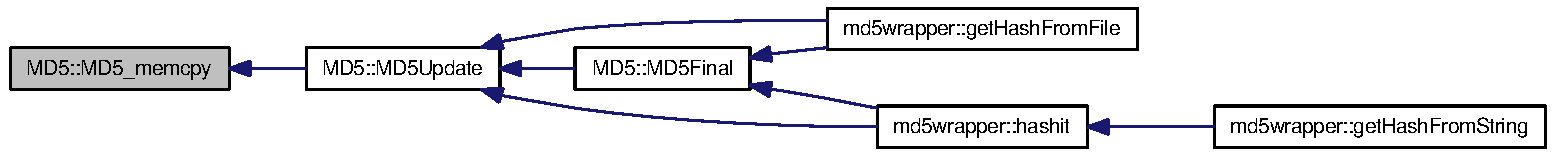
\includegraphics[width=391pt]{d7/d46/a00002_76c181f092e81df65dadf8861272ac80_icgraph}
\end{center}
\end{figure}
\hypertarget{a00002_e1a522aab83da49d1bd3f0a6f3edcd11}{
\index{MD5@{MD5}!MD5\_\-memset@{MD5\_\-memset}}
\index{MD5\_\-memset@{MD5\_\-memset}!MD5@{MD5}}
\subsubsection[{MD5\_\-memset}]{\setlength{\rightskip}{0pt plus 5cm}void MD5::MD5\_\-memset ({\bf POINTER} {\em output}, \/  int {\em value}, \/  unsigned int {\em len})\hspace{0.3cm}{\tt  \mbox{[}private\mbox{]}}}}
\label{d7/d46/a00002_e1a522aab83da49d1bd3f0a6f3edcd11}




Definicja w linii 318 pliku md5.cpp.

Here is the caller graph for this function:\nopagebreak
\begin{figure}[H]
\begin{center}
\leavevmode
\includegraphics[width=420pt]{d7/d46/a00002_e1a522aab83da49d1bd3f0a6f3edcd11_icgraph}
\end{center}
\end{figure}
\hypertarget{a00002_98039031d87c1f5b787050e2b487d83f}{
\index{MD5@{MD5}!MD5Final@{MD5Final}}
\index{MD5Final@{MD5Final}!MD5@{MD5}}
\subsubsection[{MD5Final}]{\setlength{\rightskip}{0pt plus 5cm}void MD5::MD5Final (unsigned char {\em digest}\mbox{[}16\mbox{]}, \/  {\bf MD5\_\-CTX} $\ast$ {\em context})}}
\label{d7/d46/a00002_98039031d87c1f5b787050e2b487d83f}




Definicja w linii 153 pliku md5.cpp.

Oto graf wywołań dla tej funkcji:\nopagebreak
\begin{figure}[H]
\begin{center}
\leavevmode
\includegraphics[width=270pt]{d7/d46/a00002_98039031d87c1f5b787050e2b487d83f_cgraph}
\end{center}
\end{figure}


Here is the caller graph for this function:\nopagebreak
\begin{figure}[H]
\begin{center}
\leavevmode
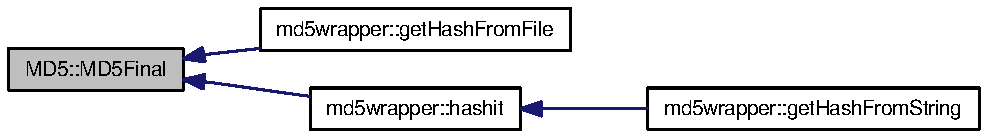
\includegraphics[width=255pt]{d7/d46/a00002_98039031d87c1f5b787050e2b487d83f_icgraph}
\end{center}
\end{figure}
\hypertarget{a00002_72b35c041cb6983aaa74e2f1c31d5a29}{
\index{MD5@{MD5}!MD5Init@{MD5Init}}
\index{MD5Init@{MD5Init}!MD5@{MD5}}
\subsubsection[{MD5Init}]{\setlength{\rightskip}{0pt plus 5cm}void MD5::MD5Init ({\bf MD5\_\-CTX} $\ast$ {\em context})}}
\label{d7/d46/a00002_72b35c041cb6983aaa74e2f1c31d5a29}




Definicja w linii 98 pliku md5.cpp.

Here is the caller graph for this function:\nopagebreak
\begin{figure}[H]
\begin{center}
\leavevmode
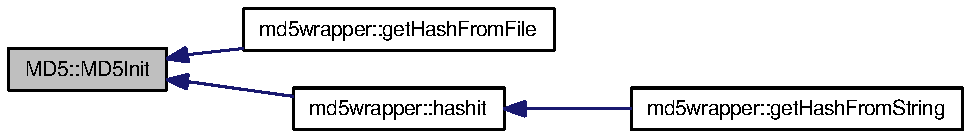
\includegraphics[width=251pt]{d7/d46/a00002_72b35c041cb6983aaa74e2f1c31d5a29_icgraph}
\end{center}
\end{figure}
\hypertarget{a00002_849ad3347bad15a23f3a40452476b1e0}{
\index{MD5@{MD5}!MD5Transform@{MD5Transform}}
\index{MD5Transform@{MD5Transform}!MD5@{MD5}}
\subsubsection[{MD5Transform}]{\setlength{\rightskip}{0pt plus 5cm}void MD5::MD5Transform (unsigned long int {\em state}\mbox{[}4\mbox{]}, \/  unsigned char {\em block}\mbox{[}64\mbox{]})\hspace{0.3cm}{\tt  \mbox{[}private\mbox{]}}}}
\label{d7/d46/a00002_849ad3347bad15a23f3a40452476b1e0}




Definicja w linii 183 pliku md5.cpp.

Oto graf wywołań dla tej funkcji:\nopagebreak
\begin{figure}[H]
\begin{center}
\leavevmode
\includegraphics[width=145pt]{d7/d46/a00002_849ad3347bad15a23f3a40452476b1e0_cgraph}
\end{center}
\end{figure}


Here is the caller graph for this function:\nopagebreak
\begin{figure}[H]
\begin{center}
\leavevmode
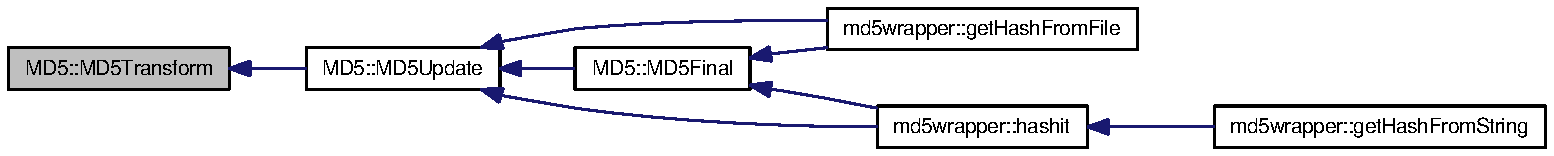
\includegraphics[width=391pt]{d7/d46/a00002_849ad3347bad15a23f3a40452476b1e0_icgraph}
\end{center}
\end{figure}
\hypertarget{a00002_a59116f0a26354a217fa186a43cd9d28}{
\index{MD5@{MD5}!MD5Update@{MD5Update}}
\index{MD5Update@{MD5Update}!MD5@{MD5}}
\subsubsection[{MD5Update}]{\setlength{\rightskip}{0pt plus 5cm}void MD5::MD5Update ({\bf MD5\_\-CTX} $\ast$ {\em context}, \/  unsigned char $\ast$ {\em input}, \/  unsigned int {\em inputLen})}}
\label{d7/d46/a00002_a59116f0a26354a217fa186a43cd9d28}




Definicja w linii 112 pliku md5.cpp.

Oto graf wywołań dla tej funkcji:\nopagebreak
\begin{figure}[H]
\begin{center}
\leavevmode
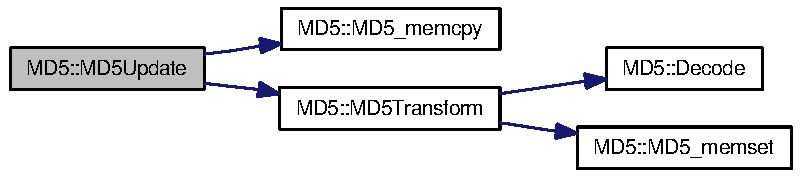
\includegraphics[width=210pt]{d7/d46/a00002_a59116f0a26354a217fa186a43cd9d28_cgraph}
\end{center}
\end{figure}


Here is the caller graph for this function:\nopagebreak
\begin{figure}[H]
\begin{center}
\leavevmode
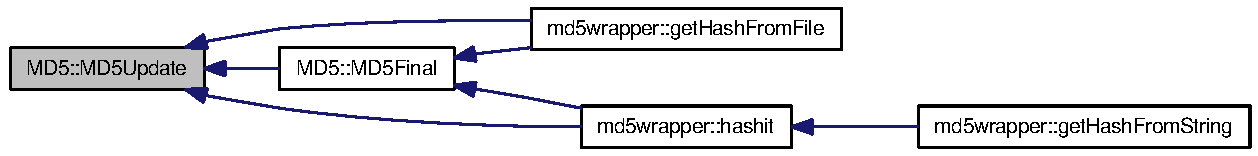
\includegraphics[width=320pt]{d7/d46/a00002_a59116f0a26354a217fa186a43cd9d28_icgraph}
\end{center}
\end{figure}


Dokumentacja dla tej klasy została wygenerowana z plików:\begin{CompactItemize}
\item 
/home/pawel/Dokumenty/Uczelnia/grupappz/Source/Ass8-server/include/md5/\hyperlink{a00010}{md5.h}\item 
/home/pawel/Dokumenty/Uczelnia/grupappz/Source/Ass8-server/include/md5/\hyperlink{a00009}{md5.cpp}\end{CompactItemize}
